\documentclass[a4paper,12pt]{article}
\usepackage[margin=19mm]{geometry}
\usepackage{amsmath,amssymb,graphicx,xcolor}
\usepackage{fontspec}
\usepackage{xepersian}
\settextfont{XB Roya}
\setlatintextfont{Latin Modern Roman}
\definecolor{ink}{HTML}{173D75}
\graphicspath{{images/}}
\setlength{\parindent}{0pt}
\setlength{\parskip}{5pt}
\linespread{1.12}
\newcommand{\qtitle}[2]{{\Large\bfseries\color{ink} پرسش \lr{#1}: #2}\par}
\newcommand{\answer}{\vfill\textbf{پاسخ یا صورت مورد تأیید و تاریخ:}\par\vspace{15mm}\hrule}
\newcommand{\sourcepage}[1]{\textbf{منبع:} نسخهٔ \lr{primary}، صفحهٔ #1 از فایل زیر.\par
\begin{LTR}\small\texttt{sources/lectures/12 Noetherian and Artinian rings.pdf}\end{LTR}}
\begin{document}
{\LARGE\bfseries پرسش‌های ابهام جلسهٔ ۱۲}\par
{\large جزوهٔ جبر پیشرفتهٔ دکتر خسروی}\par
شماره‌ها، شمارهٔ یک‌مبنای صفحهٔ پی‌دی‌اف‌اند.\par
هر سه پرسش در تاریخ \lr{2026-10-25} باز ثبت شده‌اند.\par
خوانش‌های موقت در اسلایدها مشخص‌اند. پاسخ بعدی اختیاری است؛ رونویسی متوقف نشده است.\par
\medskip\hrule\medskip

\qtitle{L12-Q01}{درجهٔ صفر در اثبات هیلبرت}
\textbf{وضعیت:} باز؛ قرارداد درجهٔ صفر و ایده‌آل چپ در اسلایدها موقت است.
\sourcepage{۲، تعریف $\varphi_n$؛ صفحهٔ ۳، کاهش درجه؛ صفحهٔ ۴، درجات کوچک؛ صفحهٔ ۵، نتیجه}
\textbf{عبارت منبع:} تعریف برای $n\in\mathbb N$ آمده، اما فهرست درجات باقی‌مانده
فقط $\varphi_1,\ldots,\varphi_{k-1}$ است.
\begin{center}
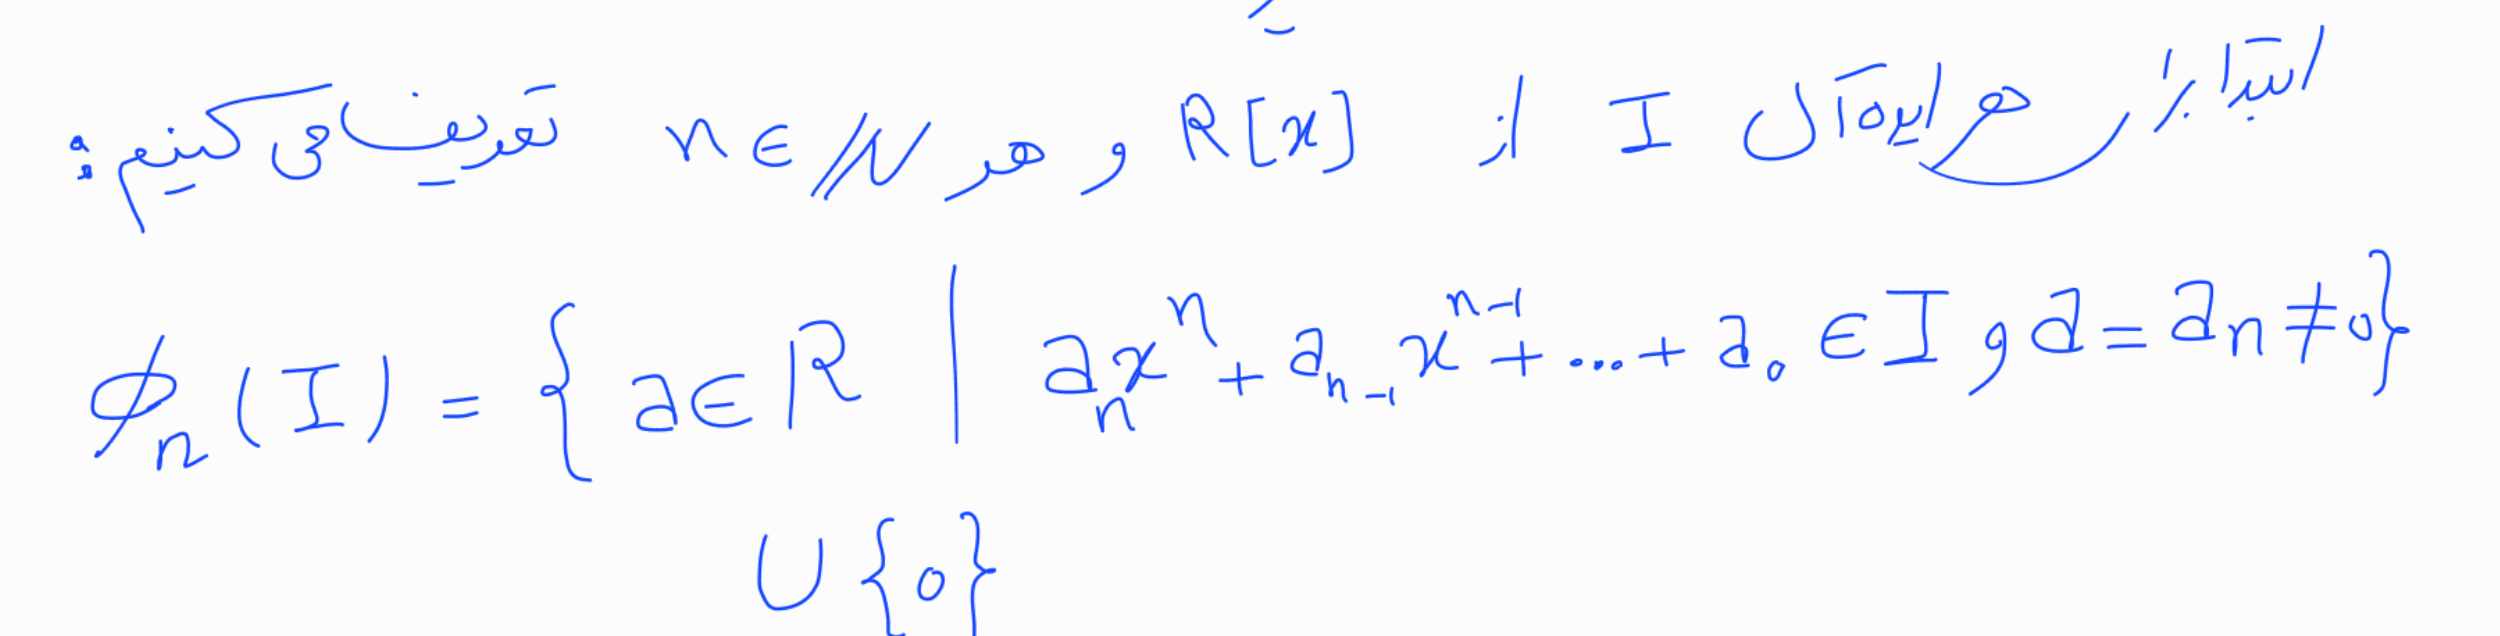
\includegraphics[width=.90\linewidth,height=48mm,keepaspectratio]{L12-Q01-definition.png}\\[3pt]
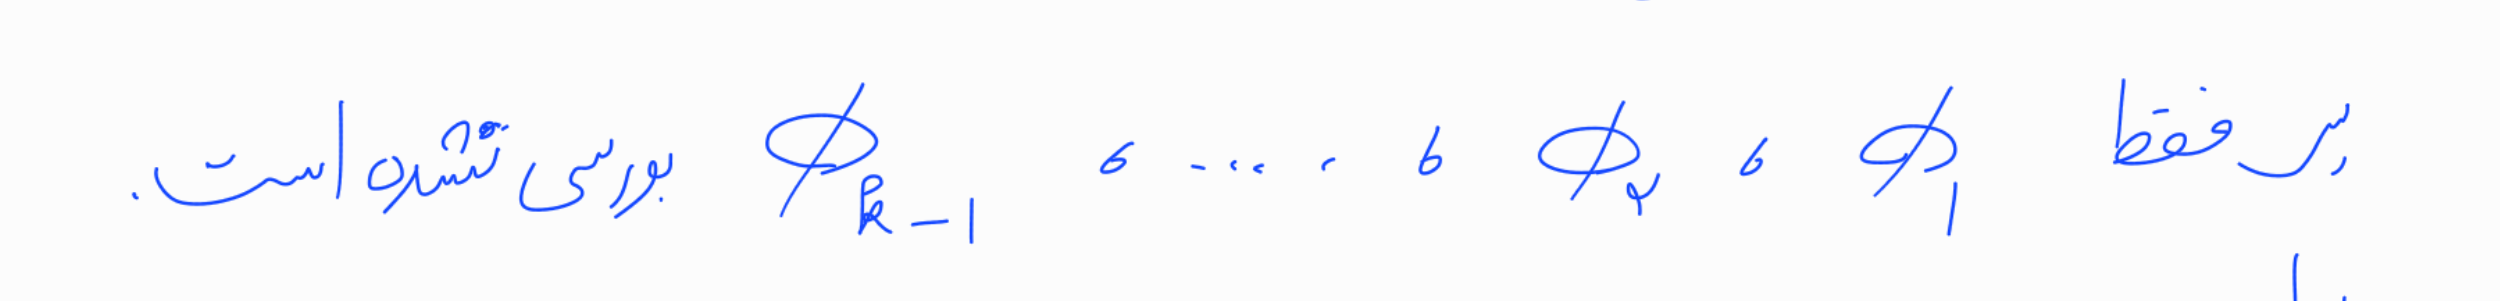
\includegraphics[width=.90\linewidth,height=30mm,keepaspectratio]{L12-Q01-low-degrees.png}
\end{center}
\textbf{ابهام و اثر آن:} اگر شاخص‌ها از ۱ شروع شوند، برابری ضرایب پیشرو در درجات مثبت
برابری ایده‌آل‌ها را تضمین نمی‌کند؛ مرحلهٔ ثابتِ کاهش درجه نیز باید پوشش داده شود.
اگر $0\in\mathbb N$ باشد، فهرست صفحهٔ ۴ ظاهراً $\varphi_0$ را جا انداخته است.

\textbf{پرسش:} آیا تعریف را برای $n\geq0$، با
$\varphi_0(I)=I\cap R$، و فهرست درجات کوچک را
$\varphi_0,\ldots,\varphi_{k-1}$ بنویسم و حالت ثابت را در کاهش درجه لحاظ کنم؟
همچنین آیا منظور از ایده‌آل‌های این اثبات، ایده‌آل‌های \textbf{چپ} است، مطابق حکم نوتری چپ؟
در خوانش موقتِ اسلایدها همین قرارداد به کار رفته؛ مرتبهٔ توقف $\varphi_0$ و شرط $m\geq\ell$ نیز صریح شده است. اگر $k=0$ باشد، درجهٔ کوچکی باقی نمی‌ماند. این تکمیل‌ها تأیید نهایی نشده‌اند.
\answer
\newpage

\qtitle{L12-Q02}{ساختار مدولی روی مجموعهٔ همریختی‌ها}
\textbf{وضعیت:} باز؛ فقط خوانش گروه جمعی به‌طور موقت در اسلاید استفاده شده است.
\sourcepage{۱۱، میانهٔ صفحه، زیر فرمول صفرشدن بلوک‌های غیرقطری}
\[
\operatorname{Hom}_R(n_iM_i,n_jM_j)
\cong\bigoplus_{1}^{n_in_j}\operatorname{Hom}_R(M_i,M_j)=0\quad(i\ne j).
\]
\begin{center}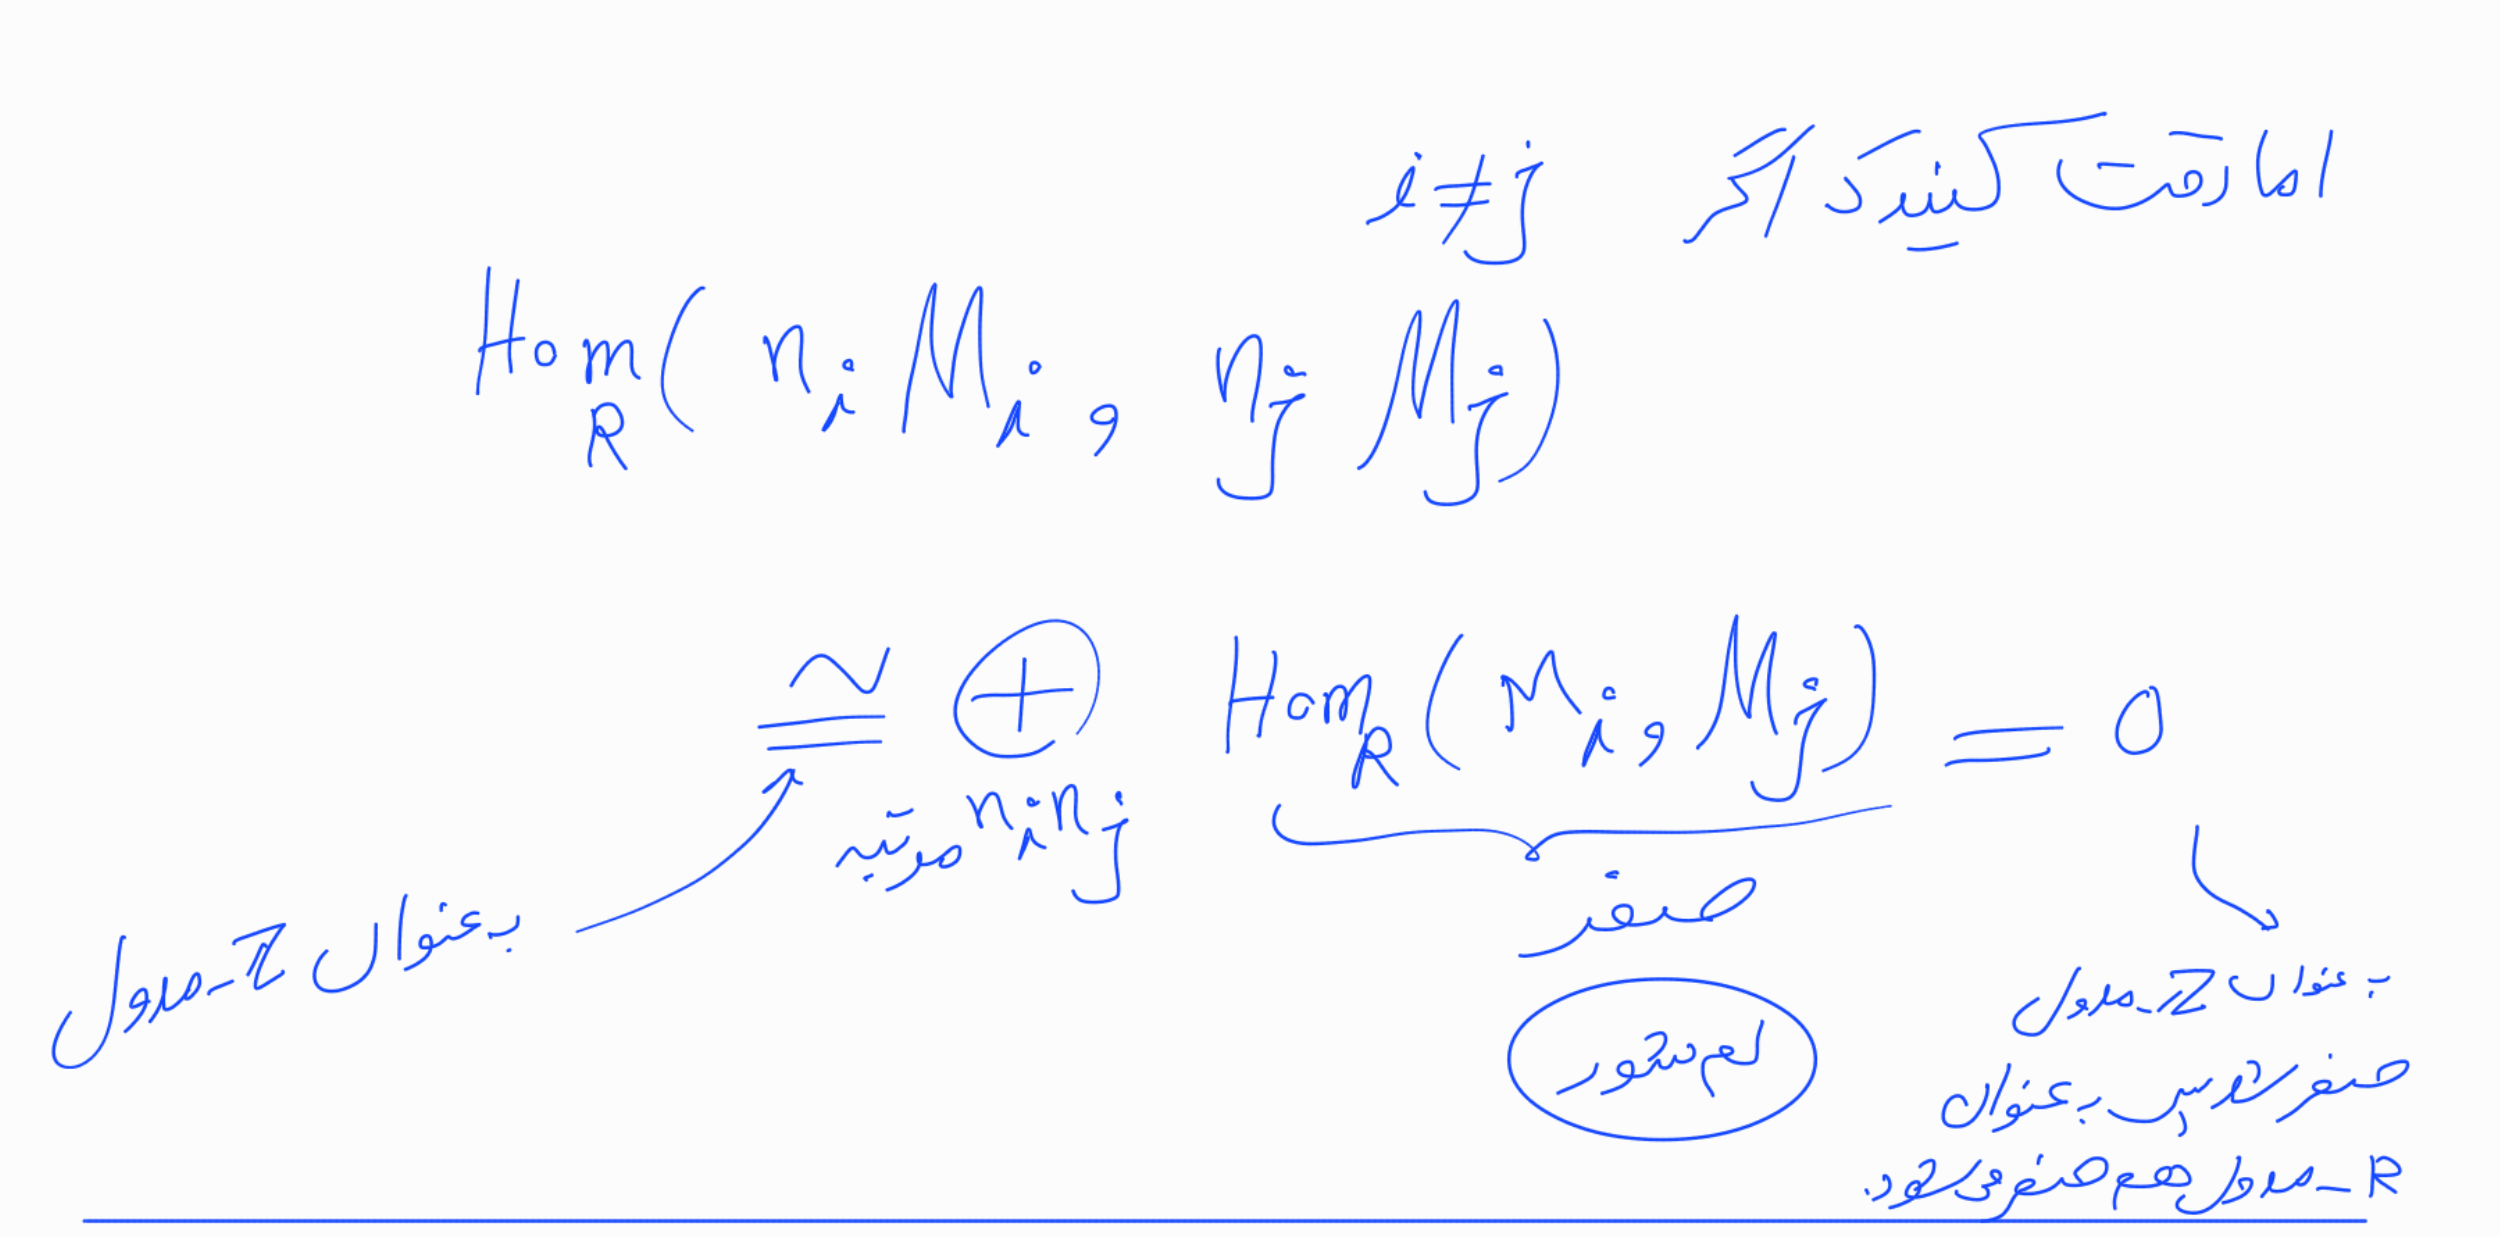
\includegraphics[width=\linewidth,height=67mm,keepaspectratio]{L12-Q02-module-structure.png}\end{center}
\textbf{عبارت منبع:} یکریختی به‌عنوان $\mathbb Z$-مدول معرفی شده و سپس گفته شده
چون به‌عنوان $\mathbb Z$-مدول صفر است، به‌عنوان $R$-مدول هم صفر است.

\textbf{ابهام و اثر آن:} برای حلقهٔ نامتبادل، مجموعهٔ
$\operatorname{Hom}_R(U,V)$ عموماً ساختار طبیعی $R$-مدول با عمل نقطه‌ای ندارد.
برای حذف بلوک‌های غیرقطری، صفر بودن گروه جمعی همریختی‌ها کافی است.

\textbf{پرسش:} آیا توضیح «به‌عنوان $R$-مدول» را حذف کنم و فقط یکریختی گروه‌های
جمعی (یا $\mathbb Z$-مدول‌ها) و صفرشدن بر اثر لم شور را نگه دارم؟
یا عمل مشخص دیگری از $R$ در این عبارت مدنظر است؟
\answer
\newpage

\qtitle{L12-Q03}{فرض یکداربودن در قضیهٔ آرتین وِدِربرن}
\textbf{وضعیت:} باز؛ فرض یکداربودن در صورت و اثبات اسلاید موقت است.
\sourcepage{۱۰، صورت قضیه و آغاز اثبات}
\begin{center}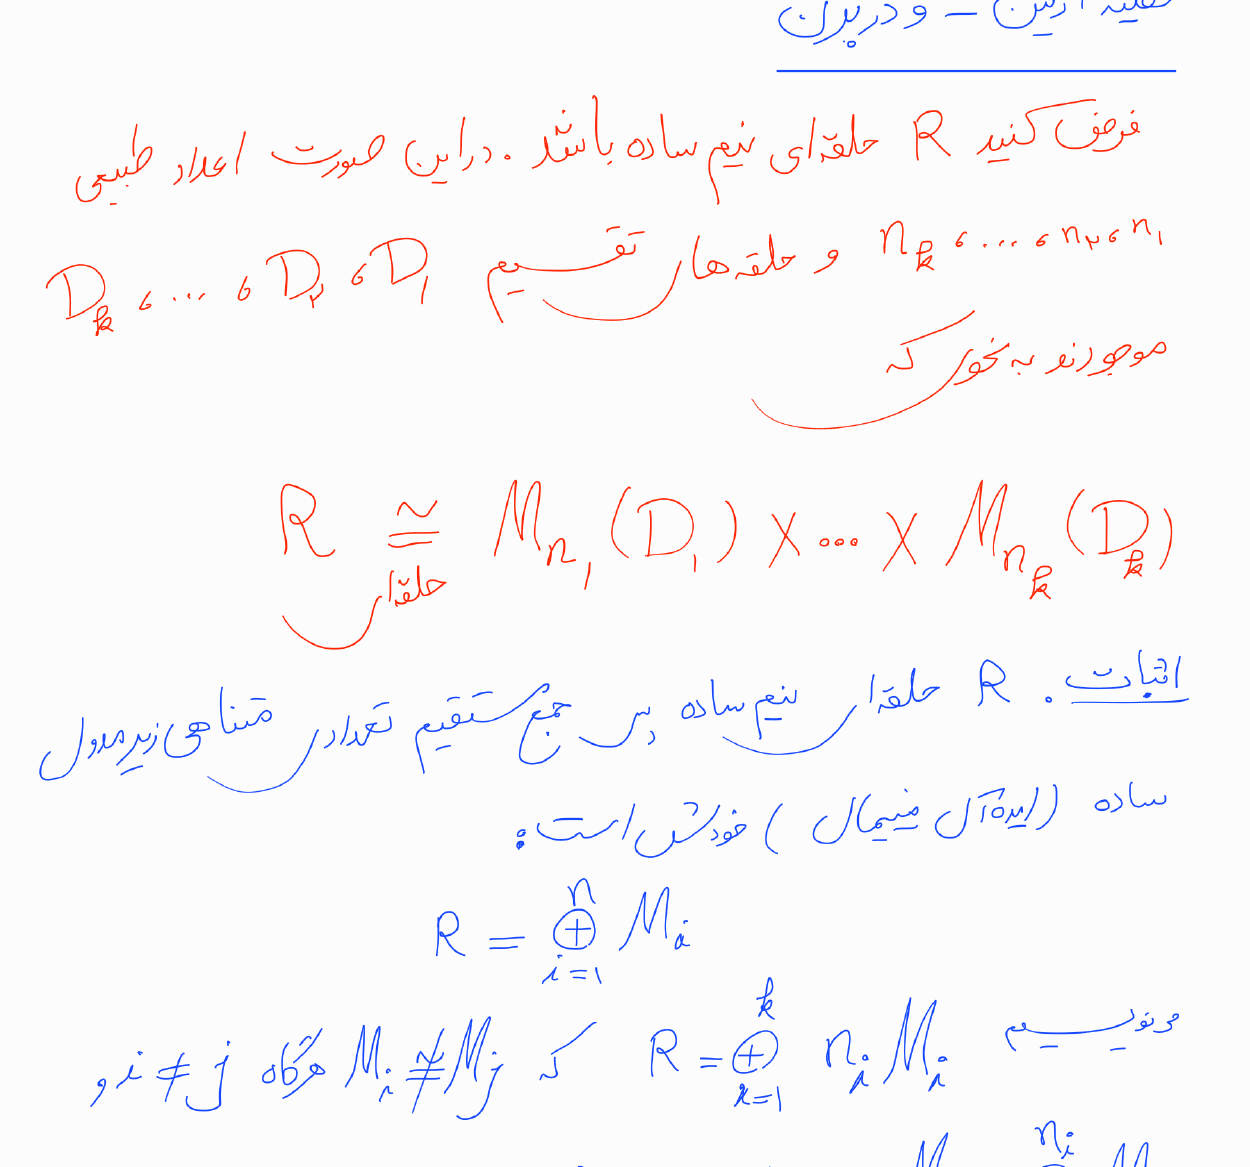
\includegraphics[width=.96\linewidth,height=86mm,keepaspectratio]{L12-Q03-unital.png}\end{center}
\textbf{عبارت منبع:} «فرض کنید $R$ حلقه‌ای نیم‌ساده باشد»؛ سپس
$R=\bigoplus_{i=1}^{n}M_i$ نوشته شده و از
$R^{\mathrm{op}}\cong\operatorname{Hom}_R(R,R)$ استفاده شده است.

\textbf{ابهام و اثر آن:} قضیهٔ اخیر در پایین صفحهٔ ۸ صریحاً برای حلقهٔ یکدار بیان شده است؛
استنتاج متناهی‌بودن تجزیهٔ حلقهٔ نیم‌ساده در جلسهٔ ۶ نیز فرض یکدار دارد.
در صورت قضیهٔ صفحهٔ ۱۰ این فرض تصریح نشده است.

\textbf{پرسش:} آیا در قضیهٔ آرتین وِدِربرن، $R$ را صریحاً
«حلقهٔ یکدار و نیم‌ساده» بنویسم؟ یا قراردادی کلی دربارهٔ یکداربودن حلقه‌های این بخش
وجود دارد که باید ثبت شود؟ صورت و اثبات با فرض صریح و موقتِ یکداربودن رونویسی شده‌اند؛ این فرض به‌عنوان تصمیم کاربر ثبت نشده است.
\answer
\end{document}
